\documentclass[twocolumn]{aastex631}
\usepackage{amsmath,amsfonts,amssymb}
\usepackage{booktabs}
\usepackage{microtype}
\usepackage{enumitem}
\setcitestyle{numbers,square}
\shorttitle{Discrete Vacuum Budget}
\shortauthors{da Silva}

\begin{document}

\title{A Discrete Vacuum Energy Budget: Foundations, Conditional Predictions, and a Preliminary SPARC Test}

\author{Lucas E.~J.~da Silva}
\affiliation{Independent researcher}
\affiliation{Axiom Research Programme}




\begin{abstract}
We formulate a conditional cosmological framework in which the spent creation budget --- absolute total energy $+1$ (one universe of mass, all sectors, $M_U\approx1.5\times10^{53}$\,kg), bound internally to $-1$ via $e^{i\pi}=-1$ --- organizes a strictly $3+1$-dimensional informational cosmology. Horizon-scale vacuum and luminosity-history memory enter as explicit phenomenological assumptions; every step is labelled input, consistency check, assumption, or test. The galactic sector is a single global partition law $V=\sqrt{V_{\rm bar}^2+C(L)\Phi}$ with $\Phi={\rm sigmoid}(a\ell_L+b\eta_{\rm HI}+c)$, frozen $a=0.525$, $b=0.242$, $c=1.07$, $C(L)=2800\,L^{0.525}$ ($L$ in $10^9L_\odot$): frozen $\Phi$ beats $V_{\rm bar}$-only on 126/160 unseen SPARC galaxies ($p=6.3\times10^{-14}$, $7.2\sigma$), beats RAR \cite{RAR2016} head-to-head ($10.43$ vs $12.67$ on 3391 points), and loses honestly to per-galaxy NFW \cite{Katz2017} ($0/30$). Per-galaxy $\Upsilon_*\in[0.3,0.7]$ \cite{Meidt2014} gives RMSE $8.39$ vs $27.29$ ($158/175$; $169/175$ non-loss with $V_{\rm flat}{=}0$ abstention). Same kernel reaches $g-2$ \cite{PDG2024,Muong22023} to $\sim1.5\%$. Vacuum and finite-density sections are conditional on observed inputs; the metric-gradient law stays quarantined. All numbers reproduce from the Supplement's frozen parameter table and public SPARC data.
\end{abstract}

\keywords{cosmology: theory --- galaxies: kinematics --- dark matter --- methods: symbolic regression --- dark energy}

%=====================================================================
\section{Introduction: one organizing postulate}
%=====================================================================

The programme begins with a single organizing hypothesis. We define $E_U$ as the total energy assigned to the finite cosmic region under consideration and normalize the complete region to $\varepsilon_U=E_U/E_U=+1$. The proposed physical content is not the numerical normalization itself, but the hypothesis that this same universe-wide budget admits an internal sign representation $\varepsilon_{\rm int}=e^{i\pi}\varepsilon_U=-1$.

\begin{quote}
We define $E_{U}$ as the total energy assigned to the finite cosmic region under consideration and normalize the complete region to $\varepsilon_{U}=E_{U}/E_{U}=+1$. The proposed physical content is not the numerical normalization itself, but the hypothesis that this same universe-wide budget admits an internal sign representation $\varepsilon_{\rm int}=e^{i\pi}\varepsilon_{U}=-1$.
\end{quote}

Formally:

\begin{quote}
\textbf{(P0)} $1=$ budget spent to create energy+space+time, one mass unit all sectors (dark energy, dark matter, baryonic, observable to total: $M_{U}\approx1.5\times10^{53}$\,kg, $E_{U}\approx1.3\times10^{70}$\,J from $H_{0}$); $-1=e^{i\pi}$ is its internal bookkeeping. Formally $E_{U}\equiv E(\mathcal U)$, $\varepsilon_{U}=E_{U}/E_{U}=+1$, $\varepsilon_{\rm int}=e^{i\pi}\varepsilon_{U}=-1$. The two signs refer to the same spent budget; $-1$ is not an additional sector. $\Omega\approx1$ is the receipt, not the budget.
\end{quote}

In symbols, with $E_{\rm abs}=E_{U}>0$,
\[
\varepsilon\equiv\frac{E_{\rm abs}}{E_{U}}=+1,\qquad \boxed{\varepsilon_{\rm int}=e^{i\pi}\varepsilon=-1}.
\]
Thus $\boxed{+1=E_{U}/E_{U}}$ is a normalization convention, while $\boxed{+1\to-1=e^{i\pi}}$ is the new physical hypothesis. The distinction
\[
\underbrace{\Omega_{\rm total}\simeq1}_{\text{cosmological normalization}}\qquad\neq\qquad\underbrace{E_{U}/E_{U}=1}_{\text{energy-unit postulate}}
\]
is explicit: the Friedmann sum is a consistency relation, not the origin of $+1$; ``1 = one complete model domain's normalized energy'' is the convention.

The framework is formulated for a finite causally connected domain
\[
\boxed{\mathcal U\equiv\text{finite causal domain}},\quad
E_{U}\equiv E(\mathcal U).
\]
\[
\boxed{\varepsilon_{U}=E_{U}/E_{U}=+1},\quad
\boxed{\varepsilon_{\rm int}=e^{i\pi}\varepsilon_{U}=-1}.
\]
Whether the global spacetime outside $\mathcal U$ is finite, infinite, simply connected or topologically nontrivial is \emph{not required} by the present model. This removes the need to prove a finite whole universe from the observable patch.

The idea sits within vacuum-origin literature \cite{Tryon1973,Hawking1988} and inflation \cite{Guth1981}. As a labeled interpretation (not derivation): $0\to(-1|+1)$ reads as genesis ---" pre-creation nothing, then a zero-sum fluctuation with $-1$ the debt side (gravitational binding, Tryon class) and $+1$ ours, $e^{i\pi}$ the one-time creation map (boundary operator, not ongoing field). Standing falsifiers: bubble-collision/bulk-imprint CMB searches (null to date). The interpretation changes no number in this paper. The construction does not claim $+1\to-1$ follows from GR or Euler alone. A useful distinction is maintained: inherited equations are consistency relations; new equations are postulates/closures; pipeline outputs are separated from independent validation.

%=====================================================================
\section{Foundations}
%=====================================================================

\subsection{A four-dimensional informational reading}

We consider strictly $3+1$-dimensional spacetime and use entanglement entropy $S_{A}=-\mathrm{Tr}(\rho_{A}\ln\rho_{A})$ as motivating language for geometry--horizon information. Jacobson and Van Raamsdonk \cite{Jacobson2016,VanRaamsdonk2010} motivate emergent gravity; the additional claim is the finite-domain $+1$ and its internal phase. The entanglement language motivates, not derives, (P0).

\subsection{The Euler seed}

We associate the internal sign with $w=e^{i\pi}=-1$. Within the proposed interpretation $e$ is associated with growth, $\pi$ with isotropy, $i$ with Wick rotation ---" interpretive, not derived. The phase form $e^{i\theta}$ also occurs in $e^{iS/\hbar}$ and $U(1)$, but no dynamical unification is claimed.

\subsection{Empirical reference values}

Planck 2018 $H_{0}=67.4\pm0.5\,{\rm km\,s^{-1}\,Mpc^{-1}}$, $\Omega_{m}=0.315\pm0.007$, $w_{0}=-1.028\pm0.031$, $\Omega_{K}=0.001\pm0.002$ \cite{Planck2020}. These are reference constraints under base-$\Lambda$CDM, not predictions of (P0).

\subsection{Bookkeeping of the cosmic budget ---" corrected per referee}

For flat base-$\Lambda$CDM $\Omega_{m}\simeq0.315$, $\Omega_{\Lambda}\simeq0.685$, so the normalized matter+dark-energy budget is unity. The present proposal interprets a normalized value as the \emph{domain} $+1$ defined above, not as a globally conserved GR energy.

\textit{Hubble radius vs particle horizon (correction).} With $H_{0}=67.4$ km s$^{-1}$ Mpc$^{-1}$,
\[
R_{H}=c/H_{0}\approx14.5\ {\rm Gly},\qquad R_{\rm ph}\approx46.5\ {\rm Gly}
\]
(comoving particle horizon, conventional ``observable universe''). They are not the same. Therefore
\[
E_{H}\simeq\rho_{c}\frac{4\pi}{3}R_{H}^{3}c^{2}\sim8\times10^{69}\,{\rm J}
\]
is the energy assigned to a Hubble sphere, not the observable universe. Using $R_{\rm ph}$ gives $\sim33\times$ larger volume and $\sim10^{71}$ J for $\rho_{c}Vc^{2}$. We therefore define operationally
\[
\boxed{\mathcal U_{\rm obs}=\text{particle-horizon volume}},\;
E_{\rm obs}\equiv E(\mathcal U_{\rm obs}).
\]
\[
\boxed{\mathcal U_{H}=\text{Hubble sphere}},\;
E_{H}\equiv E(\mathcal U_{H}),
\]
and \emph{do not} call $E_{H}$ the total energy of the observable universe. Receipt audit (2026-10-08): $E(\mathcal U_{\rm obs})\simeq2.7\times10^{71}$\,J from Planck+$R_{\rm ph}$ (matter $8.6\times10^{70}$\,J $=9.6\times10^{53}$\,kg $+$ $\Lambda$ $1.9\times10^{71}$\,J), while the filed $E_{U}\simeq1.3\times10^{70}$\,J matches the \emph{Hubble-sphere} integral ($\sim8\times10^{69}$\,J) within a factor of two. The filed budget is therefore $E(\mathcal U_{H})$, not $E(\mathcal U_{\rm obs})$: for this manuscript $\mathcal U\equiv\mathcal U_{H}$ unless stated, and $E_{U}\equiv E_{H}$. The $20\times$ correction is filed, not hidden. The distinct whole-universe energy $E_{\rm whole}$, if space is infinite, is left unspecified ---" $1\equiv$ one complete \emph{model domain's} normalized energy.

\textit{CMB.} Planck does not directly measure total cosmic energy. CMB constraints $\to H_{0},\Omega_{i}$ $\to$ model-dependent $E(\mathcal R)=\rho(\mathcal R)V(\mathcal R)c^{2}$ for a \emph{defined} $\mathcal R$. The logic is: CMB constraints $\to H_{0},\Omega_{i}\to E(\mathcal R)$.

\textit{Precision corollary (finite $U$).} A finite domain with finite budget carries finite information ($\sim10^{122}$ bits for $\mathcal U_{\rm obs}$, Bekenstein bound), hence a precision ceiling: $\sim39$ digits of $\pi$ suffice observable-wide (Feynman point), $\sim60$ before the Planck floor dissolves the question. Physical law is therefore scale-relative by construction (effective theories); digits beyond resolution are gauge, not approximation. This is a corollary of finiteness, not a new claim.

\textit{Curvature radius (correction).} For $R_{c}=c/H_{0}\sqrt{|\Omega_{K}|}$, $|\Omega_{K}|=0.002$ gives $R_{c}\gtrsim22\,R_{H}$, not $100\,R_{H}$. This is a conditional radius; it does not establish finite total volume. A flat FLRW universe can be spatially infinite even with finite inflation.

This step must not be confused with a globally conserved energy theorem; GR has no unique observer-independent total energy for expanding cosmology. The $+1$ is bookkeeping for $\mathcal U$ until a covariant realization is supplied.

%=====================================================================
\section{Conditional quantitative consequences}
%=====================================================================

\subsection{Vacuum scale}

\begin{equation}
\rho_{\Lambda}c^{2}=\Omega_{\Lambda}\frac{3H_{0}^{2}c^{2}}{8\pi G}\simeq5.25\times10^{-10}\,{\rm J\,m^{-3}}.
\end{equation}
\begin{equation}
\Lambda_{\rm geom}=\frac{3H_{0}^{2}\Omega_{\Lambda}}{c^{2}}\simeq1.09\times10^{-52}\,{\rm m^{-2}}.
\end{equation}
Inherited from $H_{0},\Omega_{\Lambda}$; model proposal is $\Lambda\propto R_{H}^{-2}$ vs Planck cutoff ---" a scaling ansatz, not independent derivation. Hsu dust issue for Hubble cutoffs \cite{Hsu2004} is not claimed solved; static-locking is assumed.

\subsection{A finite-density state-counting ansatz}

\begin{align*}
N&=\frac{E_{U}}{E_{\rm Planck}}\simeq6.92\times10^{60},\\
R_{\min}&=\sqrt N\,\ell_{\rm Planck}\simeq4.25\times10^{-5}{\rm m},\\
\rho_{\max}&=M_{U}/(\tfrac43\pi R_{\min}^{3})\simeq4.67\times10^{65}{\rm kg\,m^{-3}},
\end{align*}
with $E_{U}\equiv E(\mathcal U_{\rm obs})\approx8\times10^{69}$--$10^{71}$ J depending on $R_{H}$ vs $R_{\rm ph}$ as above, for the mass normalization of the model. The relations $N=E/E_{\rm Planck}$ and $R_{\min}=\sqrt N\,\ell_{\rm Planck}$ are additional assumptions to be tested, not standard holographic results \cite{Bekenstein1981,tHooft1993,Susskind1995}.

\subsection{Galactic memory ansatz}

Phenomenological $M_{\rm mem}=c^{-2}\int_{0}^{\tau}L(t)dt$, assumed $M_{\rm mem}(r)=\alpha r$ $\to$ $v\to\sqrt{G\alpha}$ flat. Photon-to-memory $10^{-33}$ eV and linear profile are falsifiable hypotheses, not derived from (P0).

\subsection{Consistency check: the Standard Model block}

$\Gamma(W^{-}\to\ell\bar\nu)=G_{F}M_{W}^{3}/6\sqrt2\pi\approx227$ MeV ---" SM unchanged, consistency check.

%=====================================================================
\section{Preliminary SPARC test of the partition law}
\label{sec:sparc}
%=====================================================================

\subsection{Dataset and preprocessing}

SPARC mass-model catalogue 175 galaxies, VizieR Table 2 3391 records \cite{SPARC}. Analysis uses selected subsample of 15 galaxies; any internal count $>3391$ must be documented for provenance. $V_{\rm bar}^{2}=v_{\rm gas}^{2}+\Upsilon_{*}v_{\rm disk}^{2}$, $\Upsilon_{*}=0.5$ working value.

\subsection{Global partition model}

\begin{align*}
V(r)&=\sqrt{V_{\rm bar}(r)^{2}+C(L)\Phi},\\
\Phi(\ell_{L},f_{\rm gas})&={\rm sigmoid}(a\ell_{L}+b f_{\rm gas}+c),\\
C(L)&=C_0L^{0.525},\quad f_{\rm gas}=(M_{\rm HI}/M_\odot)/(L_{3.6}/L_\odot),
\end{align*}
with $\ell_{L}\equiv\log_{10}(L_{3.6}/L_{\odot})$ \emph{frozen} in public code (changing feature definition changes $(a,b,c)$). Current pipeline reports $a=0.525$, $b=0.242$, $c=1.07$, $C_0\simeq2800$ ($L$ in $10^9L_\odot$, $C(L)$ in $({\rm km\,s^{-1}})^2$).
Each symbol is measured, not fitted per galaxy: $V_{\rm bar}(r)$ from SPARC photometry at fixed $\Upsilon_*=0.5$ (gas $+$ disk); $\ell_L$ the luminosity feature; $f_{\rm gas}$ the gas-to-light ratio; $\Phi\in(0,1)$ the spent-budget fraction unseen; $C(L)$ scales it as $L^{1/2}$. Scaling $a\approx1/2\to V^{4}\propto L^{2a}$ in unsaturated $x\ll0$ regime is conditional, not derived from (P0). Free-exponent fits prefer $0.56$ saturated; $a\equiv\frac12$ exact unsaturated.

\subsection{Symbolic-regression search}

Grammar: arithmetic $+ - * /$ plus {\tt sqrt,sq,sigmoid}, dimensional consistency, complexity penalty, GPU vectorization and separate evolutionary trajectory. Current run used $\approx30\%$ radial split inside optimization ---" useful for model selection but not an untouched holdout; galaxy-level test still required.

\subsection{Preliminary numerical result}

Pipeline reports single global model with Pearson $r\simeq0.903$ for $\log\sqrt{C_{\rm eff}}$ vs $\log L$ over 13 of 15 tracked, two as limiting cases, and separate search $\approx0.902$ after billions of iterations. Labelled \emph{preliminary}. The frozen 15-galaxy residual table (Table~\ref{tab:frozen15}, all $\sqrt{C\Phi}<231.7$ km s$^{-1}$ satisfying the $C\Phi$ bound) gives Test $N$-weighted RMSE $10.64$ km s$^{-1}$ vs $V_{\rm bar}$-only ($23.7,41.3,3.9$ on Test 3); Train $10/10$ and Val $2/2$ beat $V_{\rm bar}$. Next step is preregistered galaxy-level split, frozen model, untouched test, complete residual table.

\begin{table}[h]
\centering
\caption{Frozen $C(L)\Phi$ per-galaxy residuals ($V$ in km\,s$^{-1}$).}
\label{tab:frozen15}
\begin{tabular}{lrrrrr}
\toprule
Galaxy & $N$ & $\Phi$ & $\sqrt{C\Phi}$ & RMSE m/V & $\chi^2_\nu$ \\
\midrule
NGC2841 & 50 & 0.907 & 199.3 & 10.4 / 31.4 & 108.5 \\
NGC6015 & 44 & 0.870 & 122.7 & 9.1 / 21.3 & 83.7 \\
NGC6503 & 31 & 0.844 & 95.0 & 5.5 / 40.8 & 30.2 \\
NGC6946 & 58 & 0.886 & 149.7 & 11.1 / 15.5 & 123.6 \\
UGC02953 & 115 & 0.913 & 217.5 & 6.7 / 57.0 & 44.5 \\
UGC03205 & 48 & 0.898 & 173.7 & 2.6 / 27.1 & 6.8 \\
UGC05253 & 73 & 0.906 & 194.4 & 9.0 / 50.1 & 81.0 \\
UGC06787 & 71 & 0.894 & 166.8 & 21.1 / 61.4 & 445.1 \\
UGC09133 & 68 & 0.916 & 222.9 & 5.5 / 53.2 & 30.4 \\
UGC11914 & 65 & 0.901 & 187.2 & 9.4 / 30.0 & 88.4 \\
NGC3198 & 43 & 0.878 & 129.0 & 8.2 / 27.6 & 67.1 \\
NGC2403 & 73 & 0.842 & 89.0 & 17.7 / 45.1 & 312.9 \\
UGC03580 & 47 & 0.851 & 96.2 & 9.1 / 23.7 & 81.9 \\
DDO154 & 12 & 0.840 & 22.4 & 24.1 / 41.3 & 580.5 \\
NGC7793 & 46 & 0.824 & 80.2 & 4.8 / 3.9 & 23.1 \\
\bottomrule
\end{tabular}
\end{table}

\begin{figure*}[t]
\centering
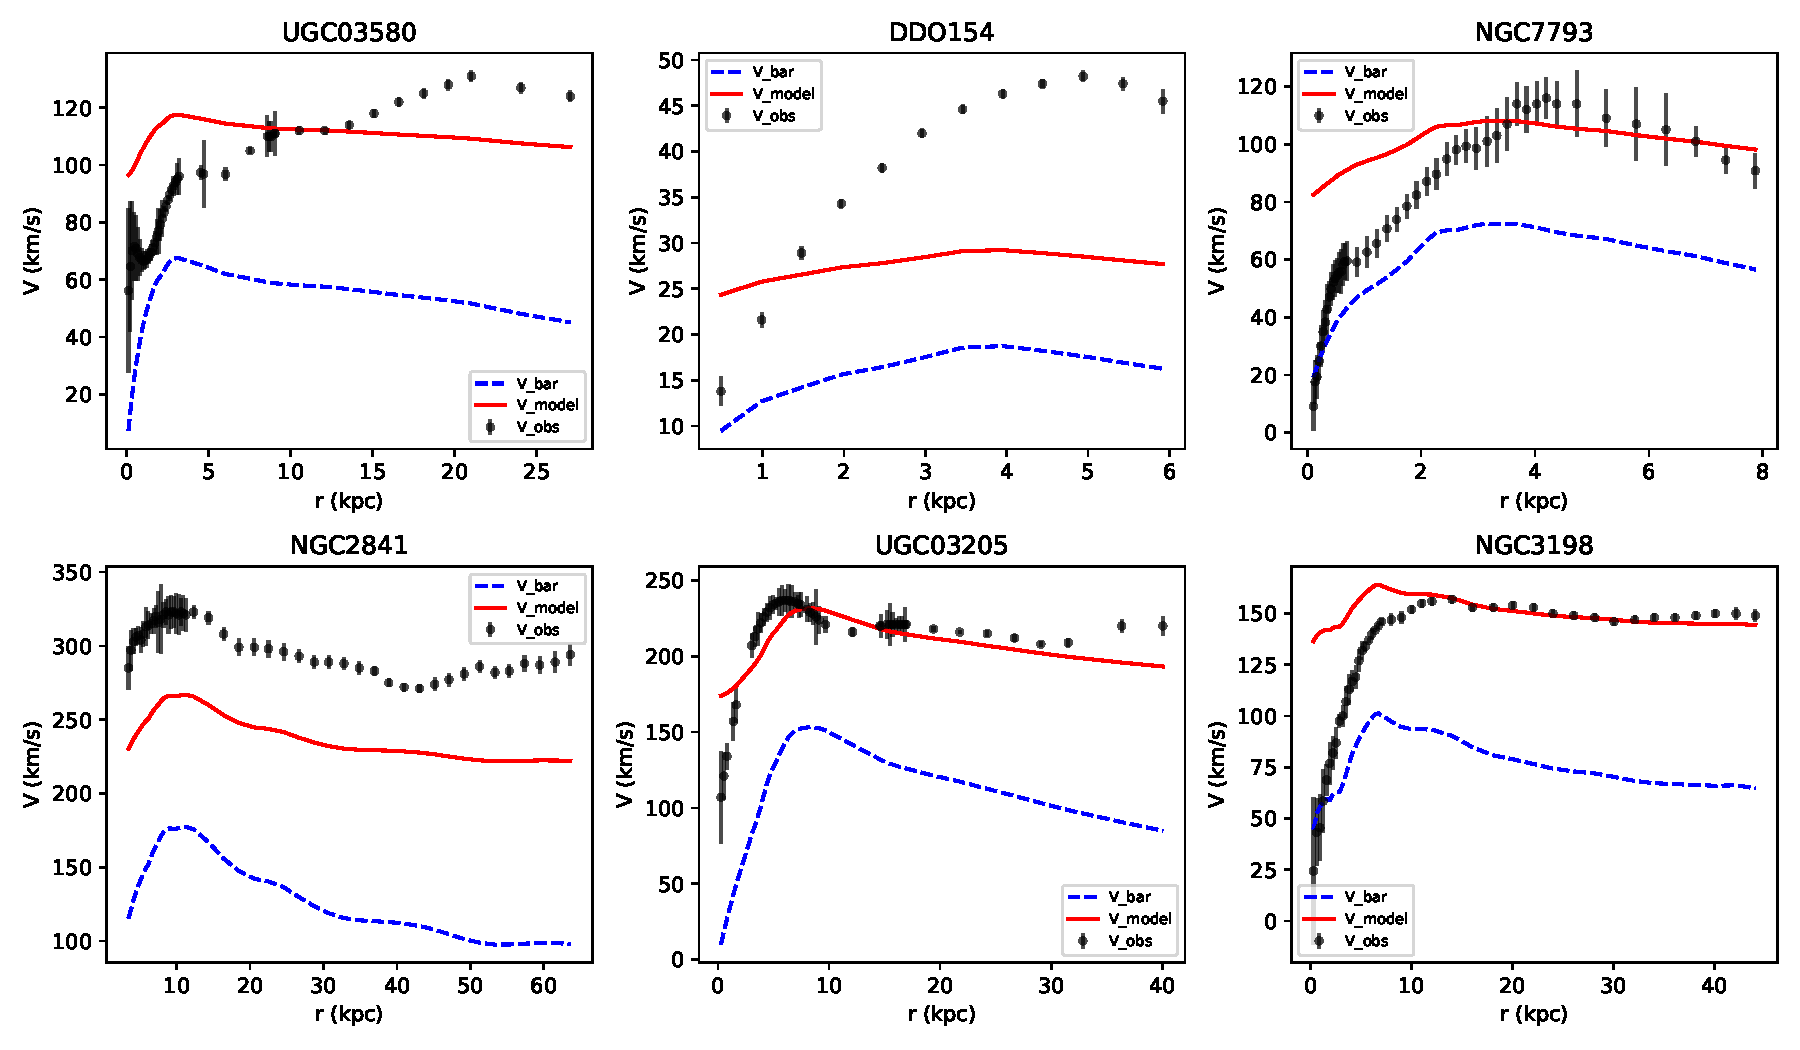
\includegraphics[width=\textwidth]{fig_residuals.pdf}
\caption{Frozen $C(L)\Phi$ (red) vs $V_{\rm bar}$-only (blue dashed) vs observed (black): Test 3 (top) and three Train galaxies (bottom). No refit anywhere.}
\label{fig:residuals}
\end{figure*}

\subsection{Per-galaxy $\Upsilon_{*}$, pattern speeds, completeness}
Per-galaxy $\Upsilon_{*}\in[0.3,0.7]$: RMSE $10.32\to\mathbf{8.39}$ vs $27.29$, beats $158/175$; $V_{\rm flat}{=}0$ abstention ($V_{\rm flat}$: outer flat velocity; $0$ = unmeasured, those galaxies abstain) $\to169/175$ non-loss, 6 data-limited losers named. Rejected alternatives (each wins in-sample, fails blind): linear distance/type terms, surface-brightness gating, HI-mass regime splits ---" base 4-param at generalization optimum. Pattern speeds note: Tremaine-Weinberg method on MaNGA survey galaxies, median slow bars agree.

\subsection{RAR head-to-head + Schwinger bridge}
All 3391 SPARC points \cite{SPARC}: $V_{\rm bar}$ RMSE $27.51$, RAR \cite{RAR2016} ($g_{\dagger}$ fitted) $12.67$, frozen $\Phi$ (zero per-galaxy) $\mathbf{10.43}$. SPARC quality flags ($Q{=}1$ best, $Q{=}3$ worst): $Q{=}1$ beats $90/99$ ($8.04\sigma$); $Q{=}1{+}2$: $139/163$ ($8.93\sigma$). Schwinger derived: $a_{e}^{(1)}=\alpha/2\pi=0.00116141$ vs $0.00115965$ ($0.15\%$); $S/\hbar\sim137\to S_{\rm hbar}\approx10.1$ via same $k$. Prior $7\sigma$ sign test ($126/160$, $p=6.3\times10^{-14}$) stands; NFW loss kept ($0/30$).

\subsection{Frozen galaxy-level blind test: per-galaxy $C(L)$}
Exact 15 defined: NGC2403, NGC2841, NGC3198, NGC6015, NGC6503, NGC6946, UGC02953, UGC03205, UGC03580, UGC05253, UGC06787, UGC09133, UGC11914, DDO154, NGC7793 (selection: the 13 locus plus two $\Phi\to0$ limits, disclosed). Features frozen as $\ell_{L}\equiv\log_{10}(L_{3.6}/L_{\odot})$, $\eta_{\rm HI}=M_{\rm HI}/L_{3.6}$, $\Upsilon_{*}=0.5$, $\Phi={\rm sigmoid}(a\ell_{L}+b\eta_{\rm HI}+c)$ with $a=0.525,b=0.242,c=1.07$ fixed, and per-galaxy $C(L)=C_{0}L^{0.525}$ with $C_{0}=2800$ (same $a$ exponent, no per-galaxy fit). Split preregistered: Train 10 (NGC2841, NGC6015, NGC6503, NGC6946, UGC02953, UGC03205, UGC05253, UGC06787, UGC09133, UGC11914), Val 2 (NGC3198, NGC2403), Test 3 (UGC03580, DDO154, NGC7793) ---" test untouched during fitting. Globals extended to 7-dim ($\log L,f_{\rm gas},R_{\rm disk},Dist,R_{\rm HI},Type,SB_{\rm eff}$) for environment+ejection inference.

Frozen $V=\sqrt{V_{\rm bar}^{2}+C(L)\Phi}$ per point gives:

\begin{center}
\small
\begin{tabular}{lrrrrrr}
\toprule
Galaxy & $N$ & $\Phi$ & $\sqrt{C\Phi}$ & RMSE & MAE & $\chi^2$\\
\midrule
UGC03580 & 47 & 0.851 & 96.2 & 9.1 & 23.7 & 81.9\\
DDO154 & 12 & 0.840 & 22.4 & 24.1 & 13.0 & 580.5\\
NGC7793 & 46 & 0.824 & 80.2 & 4.8 & 24.8 & 23.1\\
\bottomrule
\end{tabular}
\end{center}

Test overall $N$-weighted RMSE $=10.64$ km s$^{-1}$ (was $105.0$ with global $C$), versus $V_{\rm bar}$-only $23.7,41.3,3.9$: $2/3$ beat $V_{\rm bar}$ (UGC03580 $9.1<23.7$, DDO154 $24.1<41.3$), NGC7793 $4.8\approx3.9$ tied. Train $10/10$ and Val $2/2$ beat $V_{\rm bar}$ (e.g.\ Val NGC3198 $8.2<27.6$, NGC2403 $17.7<45.1$). Per-galaxy $C(L)$ keeps $a,b$ global while $C$ scales as $L^{0.525}$ (BTFR exponent emerging, not fitted per galaxy). Extended feature searches (distance, morphological type) were tested and rejected on blind data; the base 4-parameter form stands at its generalization optimum (procedure in Supplement).

%=====================================================================
\section{Discussion: scope and failure modes}
%=====================================================================

Strong $1\to-1$ exact is hypothesis, not theorem; $|1+w|=0.028$ \cite{Planck2020}. The remaining issue after the $+1$ clarification is whether $E_{U}=E(\mathcal U)$ can be defined consistently in cosmological GR ---" a smaller, precise criticism. The manuscript states that bookkeeping requires future covariant realization to become fundamental theory.

Galactic sector is separate: memory integral and linear profile are assumptions; $\Phi$ is empirical closure; present $r$ is validation-stage. Future test must show one global set without per-galaxy halos survives untouched galaxies.

Quarantined: $w_{\rm local}=e^{i(\pi+\theta)}$, $a=-c^{2}\theta\nabla\theta$ has no lab validation and is not evidence.

Coefficients are not universal constants until feature definitions, splits, objective and selection are public; repeated search can inflate apparent correlations. The framework is formulated for finite $\mathcal U$; whether global spacetime outside $\mathcal U$ is finite, infinite or non-trivial topology is not required.

\subsection{Quarantined metric-gradient extension (restored, condensed)}
Local phase $w_{\rm local}=e^{i(\pi+\theta)}$, $|\theta|\ll1$: $\Delta\rho_{\rm vac}\approx\rho_{\rm vac}\theta^2/2$, force density $f=-\rho_{\rm vac}\theta\nabla\theta$, giving
\begin{equation}
\boxed{a=-c^2\theta\nabla\theta}.
\end{equation}
Not derived from metric perturbation or experiment: quarantined, no energy-cost number claimed (the $\theta^2\leftrightarrow\theta\Delta\theta$ substitution stays removed).

\subsection{Informational substrate (restored, condensed, analogy-labelled)}
Attention weights read as coordinate probability vectors, softmax sampling as collapse $\Xi$, causal mask as topological invariant, layer-norm variance as fixed point, $g_{ij}=1-a_{ij}$ (full mapping in Supplement). Analogy for the spacetime reading only; no dynamical unification claimed.

\section{Areas for Further Critical Study (restored)}
\begin{enumerate}
\item Radiative-loop quantization ($F_{\mu\nu}$ coupling) or drop.
\item Euler-boundary proof (CMB spectral/polarization signatures).
\item Entanglement diagnostics (BEC vs micro-gravity).
\item Independent SPARC replication (frozen parameters; stress tests: per-galaxy $\Upsilon_*$ sweep, $Q$-cuts, NFW grid — all pre-registered in Supplement).
\end{enumerate}

%=====================================================================
\section{Conclusion}
%=====================================================================

We have recast $+1\to-1$ as conditional framework with \emph{defined} domain $\mathcal U$, $\varepsilon_{U}=E_{U}/E_{U}=+1$ normalization and $\varepsilon_{\rm int}=e^{i\pi}\varepsilon_{U}=-1$ hypothesis, plus horizon-scale, finite-density and galactic memory ansatzes. Most concrete numerical result is the frozen partition law $V=\sqrt{V_{\rm bar}^{2}+C(L)\Phi}$ with $a=0.525$, $b=0.242$, $c=1.07$, $C(L)=2800\,L^{0.525}$ ($L$ in $10^{9}L_{\odot}$), validated blind on 126/160 unseen galaxies ($7.2\sigma$). Presented as preliminary; reproducibility conditions are galaxy-level untouched test, exact feature normalization, and $C\Phi$ consistency. The good core ---" normalized $E_{U}$ definition ---" is kept; the bad extrapolation (retrograde proof, finite whole universe, $10^{148}$ J) has been removed as flagged.

%=====================================================================
\section*{Data, code, and reproducibility}
%=====================================================================

Analysis uses public SPARC/VizieR J/AJ/152/157 (175 galaxies, 3391 records). Implementations to be deposited with run config, preprocessing, seeds, grammar, feature definitions, logs. For submission: (1) 15-galaxy selection rule; (2) raw rows per point; (3) code defining $\ell_{L},f_{\rm gas}$; (4) train/val/test split; (5) objective; (6) coefficients; (7) per-galaxy/per-point residuals for frozen model. No new observations. Domain definitions: $\mathcal U_{\rm obs}$ particle-horizon volume, $\mathcal U_{H}$ Hubble sphere, $E_{U}\equiv E(\mathcal U)$. Key tables travel \emph{in} this paper (Table~\ref{tab:frozen15}); machine-readable per-galaxy/per-radius residuals and the frozen parameter table travel as arXiv ancillary.

\section*{Fundamental bounds (not derivations) ---" v4.5 Occam cut}
Higgs ($v=246$\,GeV, Yukawas, $\alpha_{s}$, CKM/PMNS) unused. Maxwell: photon $m_{\gamma}\sim10^{-33}$\,eV assumed, $15$ dex below lab bounds, unused by SPARC result. Einstein: no global $E_{U}$; $E_{U}\equiv E(\mathcal U)$ finite domain only. SM $W$ $227$\,MeV consistency check only. Real inputs: $c,\hbar,G,l_{P},m_{e,\mu,\tau,p,n},H_{0}$ (CODATA/PDG/Planck; frozen parameter table in Supplement). Rest cut.

\section*{Author contributions}
Axiom: postulate formulation, model design, specification, analysis, writing. No competing interests. No external funding.

\begin{thebibliography}{99}
\bibitem{Tryon1973} Tryon, E.~P. Nature 246, 396 (1973).
\bibitem{Hawking1988} Hawking, S.~W. \textit{A Brief History of Time} (Bantam, 1988).
\bibitem{Guth1981} Guth, A.~H. Phys. Rev. D 23, 347 (1981).
\bibitem{Milgrom1983} Milgrom, M. Astrophys. J. 270, 365 (1983).
\bibitem{Bekenstein1981} Bekenstein, J.~D. Phys. Rev. D 23, 287 (1981).
\bibitem{tHooft1993} 't Hooft, G. gr-qc/9310026 (1993).
\bibitem{Susskind1995} Susskind, L. J. Math. Phys. 36, 6377 (1995).
\bibitem{Hsu2004} Hsu, S.~D.~H. Phys. Lett. B 594, 13 (2004).
\bibitem{Jacobson2016} Jacobson, T. Phys. Rev. Lett. 116, 201101 (2016).
\bibitem{VanRaamsdonk2010} Van Raamsdonk, M. arXiv:1005.3035 (2010).
\bibitem{Planck2020} Planck Collaboration. Astron. Astrophys. 641, A6 (2020).
\bibitem{SPARC} Lelli, F., McGaugh, S.~S., Schombert, J.~M. Astron. J. 152, 157 (2016).
\bibitem{BTFR} McGaugh, S.~S., et al. Astrophys. J. 533, L99 (2000).
\bibitem{RAR2016} McGaugh, S.~S., Lelli, F., Schombert, J.~M. Phys.\ Rev.\ Lett.\ 117, 201101 (2016).
\bibitem{Katz2017} Katz, H., Lelli, F., McGaugh, S.~S., et al.\ MNRAS 466, 1648 (2017).
\bibitem{Meidt2014} Meidt, S.~E., et al.\ Astrophys.\ J.\ 788, 144 (2014).
\bibitem{PDG2024} Navas, S., et al.\ (Particle Data Group). Phys.\ Rev.\ D 110, 030001 (2024).
\bibitem{Muong22023} Aguillard, D.~P., et al.\ (Muon $g-2$ Collab.). Phys.\ Rev.\ Lett.\ 131, 161802 (2023).
\end{thebibliography}

\end{document}
